\documentclass[10pt]{article}
\usepackage{amsmath,amsfonts,amssymb,amsthm,amscd,enumerate}
\usepackage[utf8]{inputenc}
\usepackage[spanish,english]{babel}
\usepackage{graphicx}


\begin{document}

\section{Taller 01: Uso de comandos de shell para filtrar archivos}

Para realizar el siguiente taller dos conceptos de la biología molecular deben
tenerse en cuenta, el codigo genetico y el proceso de transcribir un mensaje
escrito en el genoma a otro llamado RNA mensajero y de este a proteina . El
primero está asociado con el desciframiento del código genético pero que es esto? En primer lugar una definición general aceptada es que un código \textit{es una combinación de caracteres que se emplea para crear y entender mensajes secretos}. ¿Cúal es el mensaje secreto en la biología?. Un tema que ha tratado de descifrar Maximo Di Giulio \cite{giulio1992}, \cite{giulio2016}
\subsection{Primera idea: El código genético}

El código genético en biología, hace parte de los muchos mensajes escritos en
el genoma (de modo basico en los genes) y que podriamos entender por analogia como el resultado de
permutaciones en matematicas, es decir se construye a partir de un término utilizado en matemáticas y probabilidad que se llama \textit{permutación con repetición}. En el caso de la  \textit{permutación con repetición} si se tienen $n$ objetos para elegir (en nuestro caso 4 nucleótidos (nuestro alfabeto estrella)) y $r$ 
maneras de elegir (en nuestro caso cada una de las 3 posiciones en el codón),
entonces la \textit{permutación con repetición} puede ser expresada asi:  $n *
n * n * \ldots (r \quad veces)$ = $n^r$. Es decir para nuestro caso, el código
genético, se puede entender como  el resultado de la siguiente permutación con
repetición expresada como $4^3$. Entonces se tienen  4 posibles caracteres
para ser asignados a la primera posición del codon, 4 para la segunda y 4 para
la tercera posición. Para una revisión actual sobre el tema consultar en
\cite{giulio2016}. Ahora esas posibles tripletas obtenidas, en la biologia
corresponderan segun unas reglas a uno o varios aminoacidos o unidades
constitutivas de las proteinas. Observe la Figura 1 para entender las reglas.
\begin{figure}[htb!]
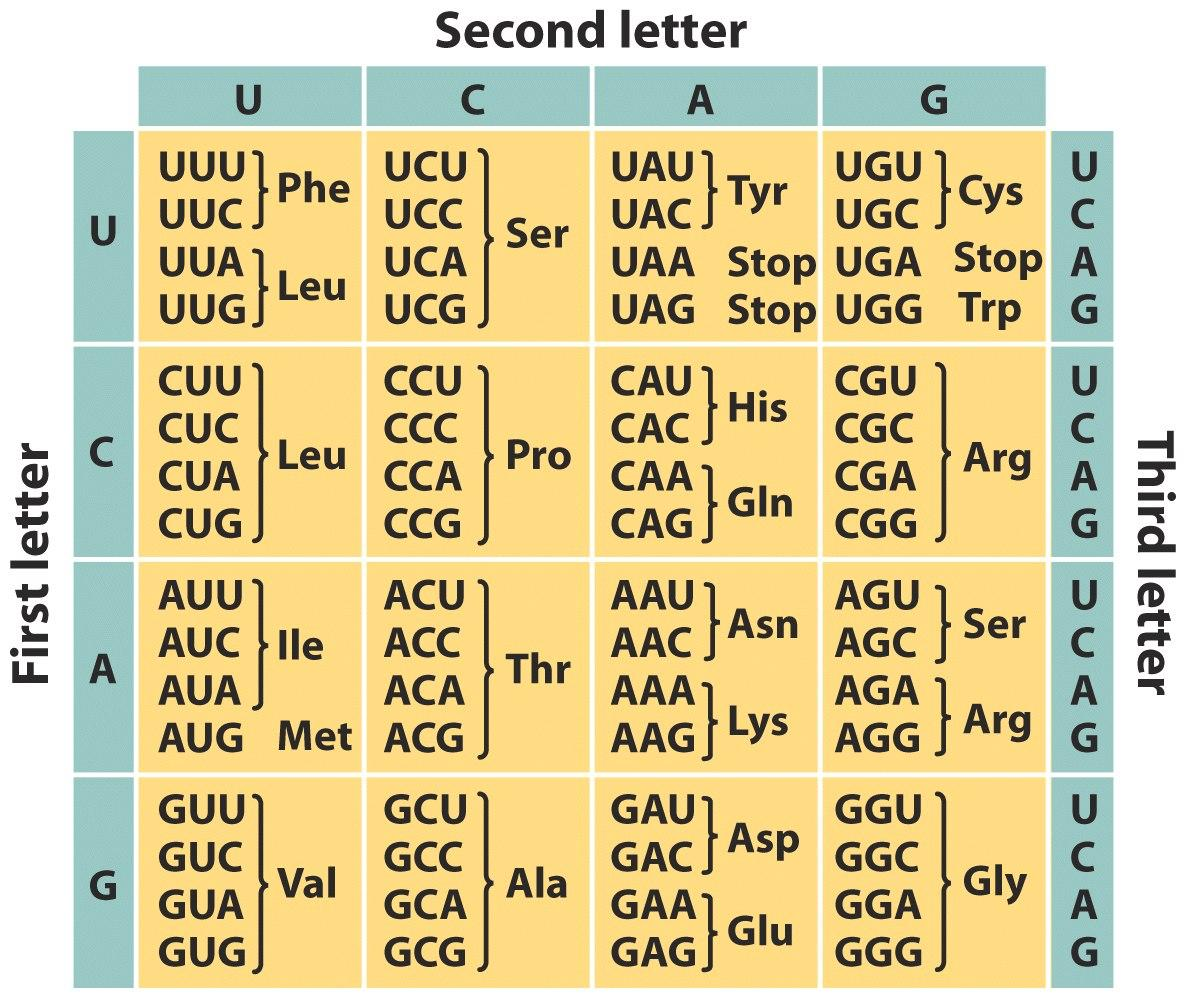
\includegraphics[scale=0.3]{./figures/code.jpg}
\caption{Tabla que respresenta la asignacion de las permutaciones con
repeticion posibles del codigo genetico y su correspondiente desciframiento a
cada tipo de aminoacido o unidad constitutiva de las proteinas}
\end{figure}

\newpage 
\subsection{Segunda idea: Molecularmente existen procesos que permitén que es a relación de tripletas (codones) sean correctamente asignadas a los aminoácidos}

En biologia el desciframiento del codigo ocurre por medio de proceso
moleculares conocidos como la transcripcion paso de la informacion del gen a
un intermediario llamado transcrito o RNA mensajero (proceso conocido com transcripcion) y
este nuevo mensaje es leido en los ribosomas para trascribir el mensaje
ecsrito en el RNA mensajero  a proteinas (proceso llamado traduccion). En la
figura 2 observe un esquema asociado.

\begin{figure}[htb!] 
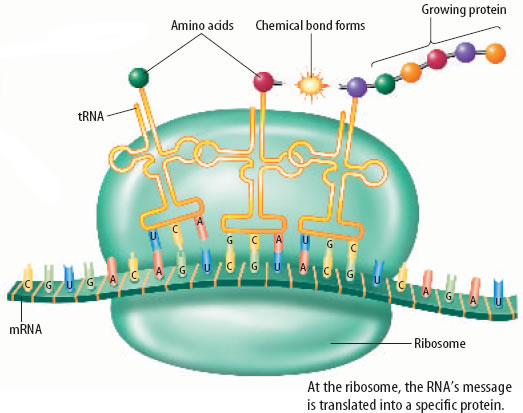
\includegraphics[scale=0.5]{./figures/translation.jpg}
\caption{Proceso de traduccion}
\end{figure}


\subsection{Introducción al lenguaje de la shell: shell programming o shell scripting}

Para comunicarnos con el sistema operativo de linux y construir scripts y tuberias de procesos (pipelines) es necesario aprender el lenguaje de la shell. La shell es referida como \textit{un intermediario entre el sistema operativo y el usuario gracias a líneas de comando que el usuario introduce. Su función es la de leer la línea de comandos, interpretar su significado y mediante instrucciones de la shell el usuario puede comunicarse con el nucleo del sistema operativo. Existen diferentes versiones como Bourne shell (sh), Almquist shell (ash), Bourne-Again shell (bash) entre otras. La shell se inicia cuando se leen las configuraciones de inicio del sistema. Posteriormente  aparece el siguiente indicador (prompt en inglés):}
equipo:/directorio/actual\$ en donde "\$" siginifica un usuario normal que no es root .

\subsection{Sintaxis general}
Para poder escribir lineas de comandos, es necesario familiarizarse con estos. Una línea de comandos es una cadena de caracteres formada por un comando que corresponde a un archivo ejecutable del sistema y tiene una sintaxis:

\begin{itemize}
\item  Sintaxis: comando $<option>$ file
\end{itemize}


\subsection {Comandos wc}
Imprime en pantalla: 1 columna número de lineas, 2 columna numero de palabras 3 número de caracteres
\subsubsection{Ejemplo}
wc ../Data/genetic\_code.txt

\subsection{tail}
Imprime las últimas 10 lineas de un archivo. Cuando hay mas de un archivo, en la salida hay un encambezamiento  dando el nombre del archivo.
\subsubsection{Ejemplo}

\begin{itemize}
\item tail -n 4 ../Data/genetic\_code.txt
\item tail -n 4 ../Data/genetic\_code.txt ../Data/genetic\_code.txt
\item tail -n 4 -v  ../Data/genetic\_code.txt ../Data/genetic\_code.txt
\end{itemize}


\subsection{cat}
Concatenación. La salida estandar "The standard output" se ve en pantalla, pero si usa el operador ($>$) se redirecciona a una nuevo archivo.
\subsubsection{Ejemplo}
\begin{itemize}
\item cat ../Data/genetic\_code.txt
\item cat ../Data/genetic\_code.txt ../Data/genetic\_code.txt
\end{itemize}

\subsection{grep}
Utilidad de la linea de comandos que busca un patrón e imprime la linea que concuerda.

\subsubsection{Ejemplo}
\begin{itemize}
\item grep ``Serine" ../Data/genetic\_code.txt
\item grep ``AA" ../Data/genetic\_code.txt
\end{itemize}

\subsubsection{Expresiones regulares}

\subsubsection{Ejemplo}
Para buscar concordancias mas complejas. Por ejemplo , solo imprima las lineas que comienzan con la letra A, seguida por cualquier otra palabra y Lys.
\begin{itemize}
\item grep  \verb"^"A.*Lys   ../Data/genetic\_code.txt ../Data/genetic\_code.txt
\end{itemize}
Para buscar concordancias mas complejas  asi como \verb"^" representa el inicio de la linea \$ representa el final de la linea

\begin{itemize}
\item  grep \verb"^"T.*Ser.*S\$ ../Data/genetic\_code.txt
\end{itemize}


\begin{itemize}

\item grep -i ine ../Data/genetic\_code.txt.  Imprime todas las lineas que contienen el patrón sin importar la letra mayuscula o minuscula. -i como argumento indica "ignore case".

\item grep -w Lysine ../Data/genetic\_code.txt. Con el comando -w se buscan coincidencias exactas de la palabra Por ejemplo "Lysine".
\item grep -v Lysine ../Data/genetic\_code.txt. El comando -v imprime todas las lineas que no coinciden con el patrón.
\item grep -E ``pattern1$|$pattern2" ../Data/genetic\_code.txt. En este caso $|$ funciona como el operador OR pero usando -E es evaluado dentro de la expresión
\item grep -E ``pattern1.*pattern2" filename. Es una alternativa para usar AND. No se tiene un operador AND in grep. Con esta idea se imprimen las lineas que contienen pattern1 y pattern2 
\item grep -E ``TCT.*Ser" genetic\_code.txt
\item grep -E ``pattern1" filename $|$ grep -E ``pattern2". Es una alternativa para simular el escenario de AND tambien, usando el pipe $|$
\item grep -E ``Ser" genetic\_code.txt  | grep -E ``AGT"
\item grep -v ``pattern1" filename. Puede usarse para negar la coincidencia del patron. Funcionaría como un operador NOT.
\end{itemize}

\subsection{echo}
Comando para la impresión de un texto, actua como la función print de otros lenguajes.

\subsubsection{Ejemplo}
\begin{itemize}
\item echo ``aaaaObbbbbbOcccccOdd"
\item echo ``aaaaObbbbbbOcccccOdd" $|$ cut -dO -f2
\end{itemize}

\subsection{cut}
Remueve campos de cada linea.

\subsubsection{Ejemplo}
\begin{itemize}
\item cut -d\, -f3 ../Data/genetic\_code.txt
\end{itemize}

\section{Combinations}

\subsection{$|$ pipe symbol}
Operador que envia la salida de una linea de comando previa a una nueva linea de comandos

\subsubsection{Ejemplo}
\begin{itemize}
\item grep ``Serine" ../Data/genetic\_code.txt $|$ cut -d\, -f3
\item echo ``aaaaObbbbbbOcccccOdd" $|$ cut -dO -f2
\item cat ../Data/genetic\_code.txt ../Data/genetic\_code.txt $|$ wc
\end{itemize}
\subsection{$>$}
Operator para enviar la salida de cat a otro archivo.
\subsubsection{Ejemplo}
\begin{itemize}
\item cat ../Data/genetic\_code.txt ../Data/genetic\_code.txt $>$ ../Results/2vecescodigo.txt
\end{itemize}

\subsection{*}

jocker, wild cart 

\section{Ejercicio}

Utilizando los comandos anteriores:
1. Cree un nuevo archivo con información de interés para usted. Archívelo solo en el directorio Data/. Indique que combinaciones y operador usted ha utilizado
2. Utilize al menos tres combinaciones de comandos para generar nueva información? 
3. Ideas de uso.

\section{Guia rápida de compilación del código fuente LATEX}

\begin{enumerate}
\item Escritura del texto científico en lenguaje LATEX (extensión .tex)
\item Escritura de la bibliografia en lenguaje LATEX (extensión .bib). \textit{Puede consultar sus articulos para converir la cita a formato bibtex consultando en http://www.bioinformatics.org/texmed/}
\item Una vex revizada la sintaxix válida para el lenguaje se procede a compilar el código asi
\begin{itemize}
\item pdflatex file.tex
\item bibtex file  \textbf{Nota: es el mismo nombre que le puso a file.tex pero sin esa extensión}
\item bibtex file
\item pdflatex file.tex (Dos o tres veces hasta que actualice la bibliografia en el arte final)
\end{itemize}
\item abrir el archivo con un visualizador de formato pdf como acroread, evince, okular, xpdf etc. Es decir evince file.pdf
\end{enumerate}
\bibliographystyle{plain}
\bibliography{guiabiblio}

\end{document}
